\documentclass[acmsmall,screen,review,anonymous]{acmart}
% ISSTA submission format (single column, 18 pages without references and the Data Availability section).
\usepackage{booktabs}
\usepackage{tikz}
\usetikzlibrary{arrows.meta,positioning,shapes.geometric,fit}
\usepackage{pgfplots}
\pgfplotsset{compat=1.17}
\setcopyright{none}
\settopmatter{printacmref=false}
\renewcommand\footnotetextcopyrightpermission[1]{}
\acmJournal{PACMSE}
\acmVolume{1}\acmNumber{ISSTA}\acmArticle{1}\acmYear{2027}\acmMonth{1}
\acmDOI{}

% ---- editing aids -------------------------------------------------------------------------------
\newcommand{\todo}[1]{\textcolor{red}{[TODO: #1]}}
% A placeholder keeps the page budget honest: a framed box of the planned height with the planned content and its data source.
\newcommand{\figph}[4]{% height, label, caption, content/source
  \begin{figure}[t]\centering
  \fbox{\parbox[c][#1][c]{0.92\linewidth}{\centering\small\textbf{FIGURE PLACEHOLDER}\\[2pt] #4}}
  \caption{#3}\label{#2}\end{figure}}
\newcommand{\tabph}[4]{% height, label, caption, content/source
  \begin{table}[t]\centering\caption{#3}\label{#2}
  \fbox{\parbox[c][#1][c]{0.92\linewidth}{\centering\small\textbf{TABLE PLACEHOLDER}\\[2pt] #4}}
  \end{table}}
\newtheorem{proposition}{Proposition}
\newtheorem{lemma}{Lemma}

\begin{document}

\title{Soundiness with Receipts: Certified Miss-Risk for Unsound Static Analyses}
\author{Anonymous Author(s)}
\renewcommand{\shortauthors}{Anonymous}

\begin{abstract}
Static taint analyses skip library code they cannot read and silently assume that no data flows through it.
A ``no leak'' verdict may therefore be wrong, and nobody says how likely that is.
We define when an analysis with a rule for trusting its clean verdicts is \emph{$(\alpha,\varepsilon)$-soundy}: with confidence $1-\varepsilon$, a new program gets a wrong clean verdict with probability at most $\alpha$.
We achieve it with receipts.
Every way data could pass through a skipped library method is a \emph{hole}; for every clean verdict a min-cut finds its \emph{receipt}, the cheapest set of assumed-absent flows it depends on; a pricer gives each flow a probability of being real, and the receipt's prices bound the chance that the verdict is wrong, the tightest such bound when only marginal probabilities are known.
The threshold on that bound is certified on whole programs with an exact test, and stays valid whatever the pricer.
On 324 Android apps, a sound over-approximation clears 72.0\% of the leak-free sinks; receipts clear 40\% of the remaining verdicts at a 5\% target, with wrong clearances in 1.0\% of held-out apps, while verdict-level conformal selection at the same target leaves a wrong clearance in half of the apps.
Because receipts name their facts, a small budget of checks pays off: verifying the 25 highest-ranked facts lifts the certified clearance to 53\% and doubles the leaks the analysis reports, while random checks do nothing.
On TaintBench malware, half of the documented leaks our analysis reaches depend on library holes, and the threshold certified on F-Droid apps transfers.
The guarantee holds for eleven pricers and four answer keys, including code-derived StubDroid summaries and a human audit; the pricers differ only in how much they clear.
We also report where the approach is weak: our analysis finds 58\% of FlowDroid's leaks and over-reports heavily, and cheap language models price too confidently to clear much.
\end{abstract}

\begin{CCSXML}
<ccs2012>
<concept><concept_id>10011007.10011074.10011099</concept_id><concept_desc>Software and its engineering~Software verification and validation</concept_desc><concept_significance>500</concept_significance></concept>
<concept><concept_id>10002978.10003022.10003023</concept_id><concept_desc>Security and privacy~Software security engineering</concept_desc><concept_significance>300</concept_significance></concept>
<concept><concept_id>10003752.10010124.10010138</concept_id><concept_desc>Theory of computation~Program reasoning</concept_desc><concept_significance>300</concept_significance></concept>
</ccs2012>
\end{CCSXML}
\ccsdesc[500]{Software and its engineering~Software verification and validation}
\ccsdesc[300]{Security and privacy~Software security engineering}
\ccsdesc[300]{Theory of computation~Program reasoning}
\keywords{static taint analysis, soundiness, library models, risk certification, Android, learn-then-test}

\maketitle

\section{Introduction}
\label{sec:intro}

Static taint analysis finds paths along which sensitive data, such as a device identifier, can reach a sink, such as a network call~\cite{flowdroid}.
On Android, these paths run through thousands of library methods whose code the analysis does not read.
Tools replace such methods with models: FlowDroid ships hand-written summaries for about 350 classes, and any method without a summary is treated as passing no data.
A ``no leak'' verdict therefore rests on assumptions about library code, and the tool does not report them.
These assumptions are not rare corner cases.
In our corpus of 324 apps, 12{,}274 of the 17{,}830 library methods that lie on source-to-sink paths have no FlowDroid model.
When FlowDroid is run without its models, 82\% of the leaks it reports disappear.
On real malware, half of the documented leaks our analysis can reach depend on library flows it does not model.
Analyses that are sound except for such documented gaps are called \emph{soundy}~\cite{soundiness}; what is missing is a way to know how often the gaps matter.

There are three common answers, and none tells the user how likely a clean verdict is to be wrong.
The first is to make the analysis sound by assuming that every unmodeled method passes all data.
This is safe but reports a flow wherever a library call could carry one: in our corpus, 28\% of the sinks that never receive sensitive data are still flagged, and nothing ranks these false alarms.
The second is to write or infer more library models, by hand, from code~\cite{stubdroid,atlas}, or with a language model~\cite{iris,semtaint}.
Every model can be wrong, and a verdict computed from a model taken as fact carries no measure of its error.
The third is to list the assumptions behind each verdict as a minimal cut in the flow graph and let a person confirm them~\cite{bastani-oopsla15}.
The list says what was assumed but not how likely each assumption is to fail, and counting the assumptions does not help: clearing every verdict that rests on a single assumption leaves a wrong clearance in 93\% of our apps.

We propose to keep the unsound analysis and attach to each clean verdict a \emph{receipt}: the smallest set of library flows the verdict assumes absent.
A \emph{pricer}, here a language model, gives each library flow a probability of being real.
The prices on a receipt add up to an upper bound on the probability that the verdict is wrong, and this bound needs no assumption about how library flows are correlated.
We show that it is the tightest bound that can be derived from the individual probabilities, and that the cheapest receipt is a minimum cut, computed by max-flow.
A verdict is accepted when its bound is below a threshold.
The threshold is not trusted but certified: we choose it on a sample of programs with an exact statistical test, so that with confidence $1-\varepsilon$, a new program receives a wrong clean verdict with probability at most $\alpha$.
We call an analysis with such a rule \emph{$(\alpha,\varepsilon)$-soundy}.

Three properties make this approach different from the answers above.
Unlike a sound analysis, it clears verdicts that depend on library code, and it ranks the rest by risk.
Unlike a model taken as fact, its error rate is measured and bounded, and the guarantee holds for any pricer, including a poor one: the quality of the prices decides how much is cleared, not whether the guarantee holds.
Unlike a list of assumptions, each receipt comes with a price, and the facts with the highest stakes can be checked first.
The guarantee is stated per program, because the user of an analysis reads one app's report; we show that the more common per-verdict error rate leaves wrong clearances in half of the apps at the same target.

We evaluate the approach on 324 Android apps from F-Droid and 33 malware apps from TaintBench~\cite{taintbench}, against four answer keys: FlowDroid's models with language-model labels for the methods it does not model, a deletion benchmark built only from FlowDroid's models, summaries generated from the Android source code with StubDroid~\cite{stubdroid}, and labels written by two language models under a written definition of a flow and checked by a person against the source code.
At a 5\% target, receipts clear 40\% of the leak-free sinks that a sound analysis cannot clear, and 1.0\% of held-out apps receive a wrong clearance.
The guarantee holds for all ten pricers and all keys we tried.
Checking the 25 receipt facts that block the most verdicts raises the cleared share to 53\% and doubles the number of real leaks the analysis reports; checking 100 random facts changes nothing.
On malware, a threshold certified on F-Droid apps gives no app a wrong clearance.

In summary, this paper makes the following contributions:
\begin{itemize}
\item A quantitative notion of soundiness, $(\alpha,\varepsilon)$-soundiness, which bounds per program how often an analysis wrongly clears a verdict.
\item Receipts with prices: a per-verdict bound on the probability of a missed flow that needs no independence assumption and is the tightest possible from marginal probabilities, together with a certified acceptance threshold that is valid for any pricer.
\item Budgeted checking: a way to choose which library facts a person should verify, without looking at any answer, so that each check clears as many verdicts as possible.
\item An evaluation on 324 benign and 33 malicious apps with four answer keys and ten pricers, receipts computed on FlowDroid itself, and an account of the cases where the approach clears little.
\end{itemize}
All code, flow graphs, prices, answer keys and audit data are available at \todo{anonymous link}.

\section{A Worked Example}
\label{sec:example}
Figure~\ref{fig:receipt} shows a verdict of the analysis on an Android app.
\begin{figure}[t]
\small
\begin{tabular}{@{}p{0.95\linewidth}@{}}
\toprule
\textbf{Sink:} \texttt{Prefs.putBoolean(String,boolean)} in \texttt{com.gianlu.dnshero}\\
\textbf{Sources:} sensitive values returned by framework calls in the same app\\
\textbf{Without library flows:} no source reaches the sink argument $\Rightarrow$ clean\\
\textbf{With every library flow on:} a source reaches it $\Rightarrow$ the verdict depends on holes\\
\textbf{Receipt:} one fact, \texttt{Boolean.valueOf(boolean)}: argument~0 $\to$ return value\\
\textbf{Price:} 0.29 \quad \textbf{Bound:} 0.29 \quad \textbf{Threshold:} 0.3 $\Rightarrow$ cleared\\
\bottomrule
\end{tabular}
\caption{A clean verdict, its receipt and its price. This verdict is one of three wrong clearances in the corpus (Section~\ref{sec:rq2}).}
\label{fig:receipt}
\end{figure}
Whether the receipt fact is real depends on the definition of a flow.
FlowDroid's summary says that boxing a boolean passes data; the real code returns one of two cached objects selected by the argument, so a code-derived key says no.
That is why the paper states a definition (Section~\ref{sec:flow}) and reports results under keys that differ on exactly such cases.

\tabph{4.2cm}{tab:facts}{The facts most accepted verdicts rest on, with their prices and what the key, the code-derived key and a person say.}{Top 10--12 facts by number of accepted verdicts (e.g.\ \texttt{Messenger.send}: 481 verdicts in 85 apps; \texttt{Bundle.putString}; \texttt{Toast.makeText}): price, key label, K2 label, human label, number of verdicts and apps. Source: \texttt{data/audit/*.csv}, \texttt{data/audit\_private/audit\_key.csv} (\textbf{have}).}

\section{Problem Setting}
\label{sec:setting}
\subsection{Holes, clean verdicts and misses}
An analysis is given as a flow graph.
Nodes are program values and heap locations, a set of source nodes, and sink nodes.
\emph{Code edges} $E_c$ are derived from code that is present.
\emph{Hole edges} $H$ are candidate library flows $x\to y$ between the arguments, receiver and return value of a framework method that has no body: for a call to a library method $m$ with arguments $a_i$, receiver $r$ and return value $v$, one candidate for every pair of endpoints that could carry data.
The \emph{unsound analysis} $A_0$ uses $E_c$ only.
A sink $t$ is \emph{clean} in $A_0$ if no source reaches it in $E_c$, and \emph{hole-dependent} if some source reaches it in $E_c\cup H$.
Let $T\subseteq H$ be the library flows that are real, unknown to the analysis; the \emph{completed analysis} $A^*$ uses $E_c\cup T$.
A clean hole-dependent verdict is a \emph{miss} if a source reaches $t$ in $E_c\cup T$.
``Wrong clearance'' means a miss relative to the answer key's $T$.
A sound over-approximation clears the sinks that are unreachable in $E_c\cup H$; the hard slice is the clean hole-dependent sinks.

\subsection{What counts as a flow}
\label{sec:flow}
A library flow from $X$ to $Y$ exists if, in ordinary executions with standard arguments, $X$'s data, a computed representation of it, or a reference to it reaches $Y$ through copying, storage or readout, including documented properties.
Mere selection or control (an index picks an element), incidental bookkeeping, and behavior that only a custom override or callback would produce do not count.
Cases that cannot be decided from the API contract remain unknown.
A negative label therefore means no transfer in this scope, not absence of every information flow; FlowDroid also has optional implicit-flow modes, which we do not use.
Keeping a reference to the argument (a queue, a retained listener) counts as a flow.
The choice matters for the audit (Section~\ref{sec:rq4}) and not for the certified clearance on this corpus.
Appendix~\ref{app:flow} gives the rubric used by the people and models that labeled facts.

\section{Approach}
\label{sec:approach}
\subsection{Receipts}
A \emph{receipt} for a hole-dependent clean sink $t$ is a set $C\subseteq H$ such that every path from a source to $t$ in $E_c\cup H$ uses an edge of $C$ (a cut).
\begin{lemma}\label{lem:cut}
If no edge of $C$ is in $T$, then no source reaches $t$ in $E_c\cup T$, so the verdict is not a miss.
\end{lemma}
\noindent The proof is immediate: any path in $E_c\cup T$ is a path in $E_c\cup H$ and would use an edge of $C$.
Receipts of the verdicts that get accepted are small: of the 11{,}312 leak-free sinks cleared at the main threshold, 63.8\% rest on one fact, 26.6\% on two and 1.8\% on five or more (over all 84{,}753 hole-dependent sinks: 28.7\%, 18.3\% and 38.3\%).
They are checkable: each fact is a statement about a named library method (``argument~0 flows into the return value of \texttt{Boolean.valueOf}'') that a person or a test can judge.

\subsection{Pricing and the bound}
A \emph{pricer} assigns each hole edge $h$ a price $p(h)\in[0,1]$, intended as $\Pr[h\in T]$.
Section~\ref{sec:impl} lists the pricers.
By Lemma~\ref{lem:cut} and the union bound, $\Pr[\text{miss}]\le\min(1,\sum_{h\in C}p(h))$ without any independence assumption.
Because several cuts may exist, we take the one of least total price, a minimum cut with capacities $p$ (code edges have infinite capacity), computed by max-flow.
\begin{proposition}\label{prop:tight}
Among all joint distributions of $T$ with marginals $\Pr[h\in T]=p(h)$, the largest probability that a source reaches $t$ in $E_c\cup T$ equals $\min(1,\mathrm{mincut}_p(t))$.
\end{proposition}
\noindent\emph{Proof.}
For any cut $C$, reachability needs an edge of $C$, so the probability is at most $\sum_{C}p$, hence at most the minimum.
Conversely, decompose a maximum flow of value $F\le 1$ into paths with flows $f_k$, and let world $k$, of probability $f_k$, contain exactly the hole edges of path $k$, padded with further edges up to the marginals, which flow conservation allows.
Every marginal is met and $t$ is reachable with probability at least $F$.\hfill$\square$

\noindent The min-cut is therefore the best bound derivable from marginals alone; a tighter bound needs knowledge of correlations, which the inference of Praline~\cite{praline} can use when it exists and which we do not have.
Section~\ref{sec:rq7} checks the proposition numerically.

\subsection{Calibrating the acceptance threshold on whole programs}
A bound is only as good as the prices; we therefore certify a threshold on the bound instead of trusting it.
A verdict is \emph{accepted} at threshold $\delta$ if its bound is at most $\delta$.
For a program $P$ let $L(P,\delta)=1$ if some accepted verdict of $P$ is a miss, and let $R(\delta)=\mathbb{E}\,L$, the probability that a new program has a wrong clearance.
$L$ is non-decreasing in $\delta$.
\begin{proposition}[Certified threshold]\label{prop:ltt}
Let $P_1,\dots,P_n$ be exchangeable with a new program, let $\delta_1<\dots<\delta_K$, and test $H_k:R(\delta_k)>\alpha$ in order with the exact binomial test of $\sum_i L(P_i,\delta_k)\sim\mathrm{Bin}(n,\alpha)$ at level $\varepsilon$.
Let $\hat\delta$ be the largest $\delta_k$ such that $H_1,\dots,H_k$ are all rejected (abstain if $H_1$ is not).
Then $\Pr[R(\hat\delta)\le\alpha]\ge 1-\varepsilon$.
\end{proposition}
\noindent This is fixed-sequence testing in the Learn-then-Test framework~\cite{lt}: the $L(P_i,\delta_k)$ are independent Bernoulli$(R(\delta_k))$, each test is exact, and a fixed sequence controls the family-wise error.
Two remarks matter for the claims.
First, \emph{validity does not depend on how the bounds were computed}: any score (a union bound, a maximum, a product) is valid after calibration; prices and the min-cut determine power and give each verdict an explanation (Section~\ref{sec:rq8}).
Second, the unit must be the program: verdicts within one app share facts and apps differ, so verdict-level selection is not valid (Section~\ref{sec:rq7}).

\subsection{What the guarantee says}
For a new app drawn like the calibration apps, with probability at least $1-\varepsilon$ over the calibration sample, the probability that an accepted clean verdict is a miss is at most $\alpha$, relative to the answer key and to the analysis $A_0$.
It does not say that $A_0$ finds the leaks FlowDroid finds, that the key is right, or that apps are exchangeable with apps of another kind (Section~\ref{sec:threats}).

\figph{6.2cm}{fig:curve}{Coverage against risk for the main pricer. Share of clean hole-dependent verdicts cleared and share of apps with at least one wrong clearance, as the threshold $\delta$ grows; the certified threshold sits before the cliff.}{Line plot over $\delta\in\{0.01,\dots,0.5\}$: cleared share (left axis) and apps with a wrong clearance (right axis), main key, Jev. Source: per-$\delta$ lines of \texttt{app\_ltt.py} (\textbf{have}: e.g.\ 3/324 apps at $\delta{=}0.3$, 135/324 at $0.5$). Also draw the same curve for the other pricers.}

\section{Implementation}
\label{sec:impl}
\paragraph{Analysis.}
Soot~\cite{soot} extracts facts from each APK (all shipped code, including bundled libraries).
A Souffl\'e~\cite{souffle} program computes a whole-app, context-insensitive, type-filtered Andersen points-to analysis with field sensitivity, and propagates taint from FlowDroid's default source list (84 sources, 193 sinks) with every hole on, restricted to the part that can still reach a sink.
Hole atoms at framework call sites come from a menu of endpoint pairs per method (argument or receiver to return value, receiver or mutable argument).
FlowDroid's manual summaries (about 350 files) give the library model of the completed analysis and one of the answer keys.
The relevant graph is stored compressed (a few MB per app), so every pricing, ablation and answer key is post-processing.

\paragraph{Min-cut.}
A min-cut is computed per sink site with max-flow.
Strongly connected groups of infinite-capacity code edges are contracted once per app; the contraction leaves bounds and receipts unchanged (identical output on all 332 apps) and makes evaluation about 25 times faster on the largest apps.

\paragraph{Pricers.}
\emph{Jev}, our first pricer, returns calibrated probabilities for yes/no questions, asked once per candidate flow with the flow rule stated (``a tainted object taints everything read or obtained from it'').
Stating the rule matters: without it, getters on a tainted receiver are priced low and wrong clearances concentrate on a few widely bundled facts (Section~\ref{sec:rq8}).
\emph{General language models} are asked for one probability per candidate flow of a method (verbalized, temperature 0): Sonnet~5 and a panel of other models (Section~\ref{sec:rq3}).
Baselines: \emph{counting} (a flat price); a \emph{frequency prior} over the package and endpoint kinds; a \emph{feature classifier} (logistic regression on method-signature features, cross-fitted by method or by class and, in deletion runs, trained without the deleted methods); and the \emph{language model's yes/no taken as fact}, the model-as-specification approach~\cite{iris,semtaint}.

\tabph{4.0cm}{tab:cost}{Cost of each step on the 8-core, 62\,GB server: graph build, evaluation, pricing (time and dollars per pricer), calibration.}{Rows: graph build (183 new graphs from 367 APKs in 14\,h), evaluation of 332 apps (3.5--7\,h before contraction; after: to measure), pricing time and cost per pricer (Jev about \$0.4; Sonnet~5 \$16.4; panel: pending), LTT 200 splits (seconds), FlowDroid per app. Source: server logs (\textbf{partly have}; panel costs pending).}

\section{Experimental Setup}
\label{sec:setup}
\paragraph{Corpus.}
We built graphs for 332 of roughly 580 downloaded F-Droid apps that fit our memory and time limits (large Kotlin and Jetpack apps do not); 324 have hole-dependent verdicts.
They contain 84{,}753 sinks whose truth the main key decides, 28{,}335 of them clean.
Apps that bundle the same libraries are not independent (Section~\ref{sec:threats}).

\tabph{3.6cm}{tab:corpus}{Corpus and graph statistics.}{Apps downloaded / built / with hole-dependent verdicts; sinks reached with all holes on (96{,}945), hole-dependent (84{,}753), clean (28{,}335), real; sink calls with a non-constant argument (169{,}700); framework methods priced (17{,}830; 12{,}274 not modeled by FlowDroid); median graph size; APK size distribution of built versus failed apps. Source: \texttt{data/scale332}, graphs, \texttt{build\_server.log} (\textbf{have}; failed-app size distribution to compute).}

\paragraph{Answer keys.}
No single key is trusted.
\begin{itemize}
\item The \emph{main key} (K3) is FlowDroid's summaries, plus Sonnet~5 labels for the methods FlowDroid does not model, so it contains model labels.
\item The \emph{deletion benchmark} (K1) takes FlowDroid's own models as truth with no model in the key: a random share of the modeled methods, or of whole classes, is deleted and becomes priced holes, and all other modeled methods stay fixed code edges.
Deleting whole classes removes the siblings a learned pricer could copy from.
\item \emph{K2} is StubDroid summaries generated from the Android~13 implementation (and from OpenJDK~8 for \texttt{java.*}); it has no model in it, covers part of the facts, and is not sound.
\item The \emph{audit}: the 446 library facts that all verdicts accepted at the chosen threshold rest on were labeled in several passes, and a person read the Android source for 67 of them (Section~\ref{sec:rq4}).
\end{itemize}

\paragraph{Protocol.}
Calibration uses 200 random half splits of the apps, $\varepsilon=0.1$, thresholds on a fixed grid ($\delta\in\{0.01,\dots,0.5\}$, finer for classifier prices), and reports the mean share of held-out apps with a wrong clearance and the mean share of clean hole-dependent verdicts cleared.
\todo{Add the spread over splits and bootstrap intervals over apps (Section~\ref{sec:rq7}).}

\section{Evaluation}
\label{sec:eval}
We ask: is unsoundness pervasive (RQ1); does priced-receipt clearing beat a sound over-approximation, and does the guarantee hold (RQ2); how do pricers compare, and does the key matter (RQ3); how good is the key behind the clearances (RQ4); how faithful is our analysis to FlowDroid (RQ5); what does it cost (RQ6); do the validity checks hold up (RQ7); which design choices matter (RQ8); does the pricer hold up on code it knows less well (RQ9); and does it matter for real leaks (RQ10).

\subsection{RQ1: Is unsoundness pervasive?}
\label{sec:rq1}
Of the 17{,}830 framework methods on source-to-sink paths, 12{,}274 are not modeled by FlowDroid.
We ran FlowDroid on 40 random small apps with and without its library summaries (\texttt{-tw NONE}).
In the 29 apps where neither run was cut short, FlowDroid reports 20 leaking sink methods with summaries and 2 without; over 36 apps 54 of 63 (86\%) leaks vanish, and none appears only without the summaries (Table~\ref{tab:fd-none}).
This is the extreme case: it measures how much a library model matters, not what FlowDroid misses with its default summaries.
\tabph{4.4cm}{tab:fd-none}{FlowDroid with and without its library summaries on the same apps.}{Per-app table or summary rows: leaking sink methods with summaries, without, only-with, only-without; complete versus partial runs. \textbf{Have} for 40 apps (36 with both answers); \textbf{scheduled}: 40 more apps to reach 80 (tighter interval).}

\subsection{RQ2: Does it clear more than a sound analysis, and does the guarantee hold?}
\label{sec:rq2}
A sound over-approximation (every hole is a flow) clears 72.0\% of the 101{,}090 leak-free sinks with a non-constant argument; the remaining 28.0\% are the hard slice.
Table~\ref{tab:main} shows what priced receipts clear of it, and Figure~\ref{fig:curve} the whole trade-off.
\begin{table}[t]
\caption{Main key, 324 apps. Share of the 28{,}335 clean hole-dependent verdicts cleared, and held-out apps with a wrong clearance (in brackets), by target $\alpha$.}
\label{tab:main}
\small
\begin{tabular}{@{}lccc@{}}
\toprule
Pricer & $\alpha{=}0.10$ & $\alpha{=}0.05$ & $\alpha{=}0.02$\\
\midrule
Counting (flat price) & 0\% & 0\% & --\\
Frequency prior & 9.2\% (4.9\%) & 6.6\% (0.8\%) & --\\
Feature classifier & 33.2\% (5.4\%) & 22.0\% (0.7\%) & --\\
Sonnet~5 probabilities & 53.0\% (5.6\%) & 29.6\% (2.5\%) & --\\
Jev & 40.0\% (1.0\%) & 40.0\% (1.0\%) & 33.4\% (0.3\%)\\
\bottomrule
\end{tabular}
\end{table}
\begin{figure}[t]
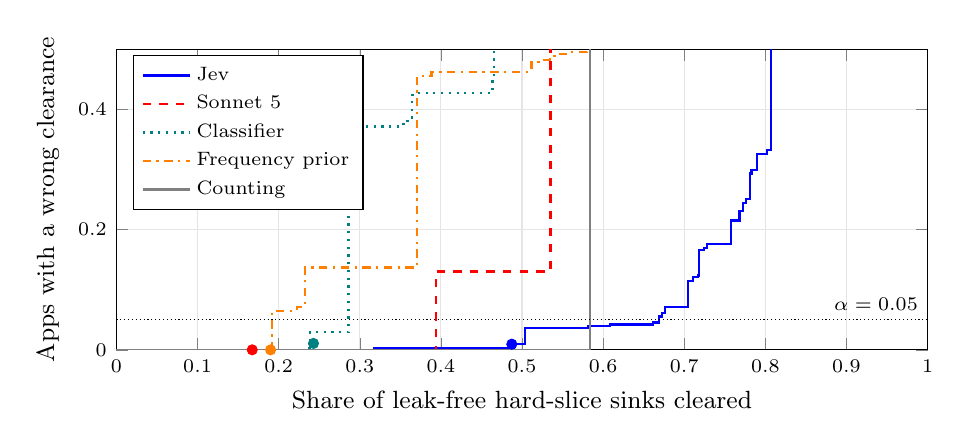
\begin{tikzpicture}
\begin{axis}[width=0.98\linewidth, height=5.4cm, xmin=0, xmax=1, ymin=0, ymax=0.5,
  xlabel={Share of leak-free hard-slice sinks cleared}, ylabel={Apps with a wrong clearance},
  legend style={font=\scriptsize, at={(0.02,0.98)}, anchor=north west}, legend cell align=left,
  tick label style={font=\scriptsize}, label style={font=\small}, grid=major, grid style={gray!20}]
\addplot[blue, thick, const plot mark left] coordinates {(0.0002,0.0000) (0.0605,0.0000) (0.0827,0.0000) (0.0921,0.0000) (0.1181,0.0000) (0.1841,0.0000) (0.1897,0.0000) (0.1965,0.0000) (0.2407,0.0000) (0.2520,0.0000) (0.2762,0.0000) (0.2994,0.0000) (0.3050,0.0000) (0.3118,0.0000) (0.3180,0.0033) (0.3261,0.0033) (0.3355,0.0033) (0.3520,0.0033) (0.3597,0.0033) (0.3755,0.0033) (0.4735,0.0033) (0.4902,0.0098) (0.5009,0.0098) (0.5032,0.0358) (0.5102,0.0358) (0.5233,0.0358) (0.5820,0.0391) (0.5871,0.0391) (0.5936,0.0391) (0.6010,0.0391) (0.6087,0.0423) (0.6149,0.0423) (0.6450,0.0423) (0.6527,0.0423) (0.6610,0.0456) (0.6685,0.0554) (0.6721,0.0619) (0.6760,0.0717) (0.7044,0.1140) (0.7110,0.1205) (0.7170,0.1238) (0.7185,0.1661) (0.7241,0.1694) (0.7285,0.1759) (0.7580,0.2150) (0.7666,0.2150) (0.7680,0.2313) (0.7728,0.2443) (0.7760,0.2508) (0.7802,0.2508) (0.7807,0.2932) (0.7830,0.2997) (0.7900,0.3257) (0.7994,0.3257) (0.8018,0.3322) (0.8065,0.8208) (0.8082,0.8274) (0.8133,0.8339) (0.8182,0.8339) (0.8347,0.8371) (0.8394,0.8534) (0.8469,0.8567) (0.8750,0.8567) (0.8798,0.8632) (0.8821,0.8697) (0.8847,0.8762) (0.8917,0.8827) (0.9022,0.8860) (0.9205,0.8860) (0.9270,0.8860) (0.9336,0.8860) (0.9522,0.8860) (0.9590,0.8860) (0.9665,0.8860) (0.9716,0.8860) (0.9774,0.8860) (0.9831,0.8893) (0.9878,0.8925) (0.9919,0.8958) (0.9955,0.9251) (1.0000,0.9349)};
\addlegendentry{Jev}
\addplot[red, thick, dashed, const plot mark left] coordinates {(0.0000,0.0000) (0.1674,0.0000) (0.3939,0.1303) (0.4285,0.1303) (0.5350,0.8078) (0.5918,0.8111) (0.6068,0.8111) (0.6350,0.8111) (0.6608,0.8111) (0.6805,0.8111) (0.6948,0.8404) (0.7063,0.8404) (0.7202,0.8436) (0.7305,0.8436) (0.7356,0.8436) (0.7433,0.8436) (0.8195,0.8436) (0.8274,0.8436) (0.8509,0.8436) (0.8554,0.8436) (0.8637,0.8436) (0.8687,0.8469) (0.8772,0.8469) (0.8823,0.8469) (0.9109,0.8469) (0.9184,0.8469) (0.9287,0.8534) (0.9332,0.8534) (0.9383,0.8534) (0.9545,0.8534) (0.9616,0.8567) (0.9902,0.8567) (0.9910,0.8664) (0.9987,0.8827) (0.9998,0.8925) (1.0000,0.9349)};
\addlegendentry{Sonnet~5}
\addplot[teal, thick, dotted, const plot mark left] coordinates {(0.0000,0.0000) (0.2307,0.0000) (0.2351,0.0033) (0.2382,0.0293) (0.2804,0.0293) (0.2862,0.0293) (0.2862,0.3648) (0.2879,0.3713) (0.3539,0.3811) (0.3637,0.3811) (0.3646,0.4235) (0.3693,0.4267) (0.3750,0.4267) (0.4184,0.4267) (0.4635,0.4528) (0.4650,0.5342) (0.4710,0.5342) (0.4754,0.5342) (0.4757,0.5440) (0.4819,0.5440) (0.5784,0.5472) (0.5829,0.5472) (0.5867,0.5570) (0.5920,0.5570) (0.6002,0.5668) (0.6049,0.5668) (0.6166,0.5668) (0.6190,0.5831) (0.6205,0.6026) (0.6252,0.6091) (0.6329,0.6091) (0.6401,0.6091) (0.6454,0.6091) (0.6516,0.6124) (0.7302,0.6124) (0.7382,0.6124) (0.7439,0.6124) (0.7456,0.6319) (0.7591,0.6352) (0.7649,0.6515) (0.7713,0.6515) (0.7806,0.6515) (0.7868,0.6515) (0.7909,0.6547) (0.8012,0.6547) (0.8041,0.6678) (0.8063,0.6808) (0.8084,0.7948) (0.8125,0.7948) (0.8197,0.7948) (0.8261,0.7980) (0.8304,0.8436) (0.8349,0.8436) (0.8413,0.8436) (0.8481,0.8436) (0.8541,0.8436) (0.8595,0.8502) (0.8637,0.8502) (0.8695,0.8502) (0.8744,0.8502) (0.8751,0.8599) (0.8825,0.8664) (0.8939,0.8664) (0.9022,0.8697) (0.9077,0.8697) (0.9107,0.8795) (0.9124,0.9023) (0.9259,0.9055) (0.9304,0.9088) (0.9387,0.9088) (0.9622,0.9088) (0.9667,0.9186) (0.9964,0.9186) (0.9977,0.9251) (1.0000,0.9349)};
\addlegendentry{Classifier}
\addplot[orange, thick, dashdotted, const plot mark left] coordinates {(0.0053,0.0000) (0.0651,0.0000) (0.0696,0.0000) (0.0754,0.0000) (0.1140,0.0000) (0.1841,0.0000) (0.1897,0.0000) (0.1922,0.0651) (0.2131,0.0651) (0.2228,0.0717) (0.2319,0.0717) (0.2320,0.1368) (0.3706,0.4560) (0.3795,0.4560) (0.3883,0.4625) (0.4882,0.4625) (0.5105,0.4625) (0.5109,0.4691) (0.5117,0.4788) (0.5220,0.4788) (0.5269,0.4821) (0.5342,0.4886) (0.5401,0.4919) (0.5476,0.4919) (0.5560,0.4951) (0.5799,0.5179) (0.5848,0.5179) (0.6408,0.5212) (0.6470,0.5212) (0.6502,0.5342) (0.6506,0.5407) (0.6566,0.5407) (0.6615,0.5440) (0.6642,0.6026) (0.6707,0.6026) (0.6794,0.6156) (0.6929,0.6156) (0.7021,0.6254) (0.7161,0.6254) (0.7194,0.6450) (0.7226,0.6580) (0.7268,0.6612) (0.7279,0.6678) (0.7381,0.6710) (0.7420,0.6775) (0.7488,0.7068) (0.7529,0.7068) (0.7563,0.7166) (0.7580,0.7655) (0.7621,0.7687) (0.7681,0.7785) (0.7736,0.7818) (0.7830,0.7915) (0.7901,0.8697) (0.7943,0.9088) (0.8409,0.9088) (0.8490,0.9088) (0.8556,0.9121) (0.8599,0.9121) (0.8881,0.9121) (0.8968,0.9121) (0.9011,0.9121) (0.9062,0.9186) (0.9127,0.9186) (0.9133,0.9251) (0.9186,0.9251) (0.9285,0.9251) (0.9383,0.9251) (0.9466,0.9251) (0.9603,0.9251) (0.9663,0.9283) (0.9712,0.9283) (0.9795,0.9283) (0.9846,0.9283) (0.9866,0.9349) (0.9919,0.9349) (0.9996,0.9349)};
\addlegendentry{Frequency prior}
\addplot[gray, thick, const plot mark left] coordinates {(0.0000,0.0000) (0.5835,0.8664) (0.7390,0.8860) (0.8466,0.8893) (0.8862,0.9283) (0.9041,0.9349) (0.9297,0.9349) (0.9440,0.9349) (0.9502,0.9349) (0.9720,0.9349) (0.9780,0.9349) (0.9851,0.9349) (0.9915,0.9349) (0.9968,0.9349)};
\addlegendentry{Counting}
\addplot[only marks, mark=*, mark size=1.8pt, blue, forget plot] coordinates {(0.4874,0.0094)};
\addplot[only marks, mark=*, mark size=1.8pt, red, forget plot] coordinates {(0.1674,0.0000)};
\addplot[only marks, mark=*, mark size=1.8pt, teal, forget plot] coordinates {(0.2429,0.0107)};
\addplot[only marks, mark=*, mark size=1.8pt, orange, forget plot] coordinates {(0.1900,0.0000)};
\addplot[black, densely dotted, forget plot] coordinates {(0,0.05) (1,0.05)};
\node[font=\scriptsize, anchor=south east] at (axis cs:1,0.05) {$\alpha=0.05$};
\end{axis}
\end{tikzpicture}

\caption{Risk against coverage on all 324 apps (main key) as the threshold grows. Dots: mean certified operating point at $\alpha=0.05$ over 200 half splits. Counting stays on the vertical axis: any threshold that clears something puts a wrong clearance in most apps.}
\label{fig:curve}
\end{figure}
At the certified thresholds, receipts clear 40\% of the hard slice at $\alpha=0.05$ with 1.0\% of held-out apps wrong; with the sound part, 83.2\% of all leak-free sinks against 72.0\%.
The observed error stays below $\alpha$ for every pricer, as the theory predicts, while the power differs by a factor of six (0\% to 40\% at $\alpha=0.05$).
Counting the assumptions is unsafe even at one fact: clearing every receipt of size one gives a wrong clearance in 93\% of the apps.
The three wrong clearances at the chosen threshold come from three different facts and apps, not from one widely bundled fact (Figure~\ref{fig:receipt}).

\subsection{RQ3: How do pricers compare, and does the key matter?}
\label{sec:rq3}
Table~\ref{tab:keys} repeats the main pricers under the other keys, and Figure~\ref{fig:deletion} shows the deletion benchmark as more classes are removed.
\begin{table}[t]
\caption{Other keys. Share cleared at $\alpha=0.05$ (held-out apps with a wrong clearance). Deletion: whole classes removed, 3 seeds.}
\label{tab:keys}
\small
\begin{tabular}{@{}lcccc@{}}
\toprule
Key & Jev & Sonnet~5 & Classifier & LLM as fact\\
\midrule
Audited (324 apps) & 39.4\% (2.0\%) & -- & -- & --\\
K2, code-derived (322 apps) & 25.7\% (1.7\%) & 33.6\% (2.3\%) & 20.4\% (2.3\%) & 38.5\% (2.5\%)\\
Deletion, 25\% of classes & 52.2\% (0.8\%) & 81.9\% (0.5\%) & 71.4\% (1.6\%) & 79.8\% (1.2\%)\\
Deletion, 75\% of classes & 50.9\% (1.3\%) & 79.1\% (1.0\%) & 33.1\% (0.5\%) & --\\
\bottomrule
\end{tabular}
\end{table}
\begin{figure}[t]
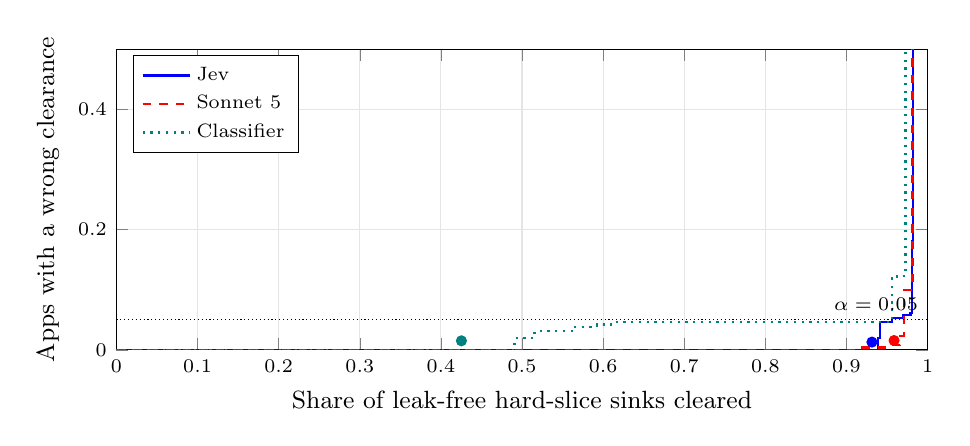
\begin{tikzpicture}
\begin{axis}[width=0.98\linewidth, height=5.4cm, xmin=0, xmax=1, ymin=0, ymax=0.5,
  xlabel={Share of leak-free hard-slice sinks cleared}, ylabel={Apps with a wrong clearance},
  legend style={font=\scriptsize, at={(0.02,0.98)}, anchor=north west}, legend cell align=left,
  tick label style={font=\scriptsize}, label style={font=\small}, grid=major, grid style={gray!20}]
\addplot[blue, thick, const plot mark left] coordinates {(0.0008,0.0000) (0.2407,0.0000) (0.3207,0.0000) (0.4006,0.0000) (0.4068,0.0000) (0.4208,0.0000) (0.4332,0.0000) (0.4387,0.0000) (0.4457,0.0000) (0.4519,0.0000) (0.4674,0.0000) (0.4759,0.0000) (0.8634,0.0000) (0.8960,0.0000) (0.9006,0.0000) (0.9154,0.0000) (0.9216,0.0000) (0.9262,0.0000) (0.9332,0.0000) (0.9387,0.0000) (0.9387,0.0192) (0.9410,0.0345) (0.9410,0.0460) (0.9457,0.0460) (0.9534,0.0460) (0.9565,0.0536) (0.9643,0.0536) (0.9697,0.0575) (0.9790,0.0613) (0.9806,0.0881) (0.9806,0.0958) (0.9806,0.1111) (0.9806,0.1801) (0.9821,0.6552) (0.9845,0.6667) (0.9845,0.6935) (0.9891,0.6973) (0.9899,0.7280) (0.9946,0.7318) (0.9953,0.7548) (0.9961,0.8506) (1.0000,0.8582) (1.0000,0.8736) (1.0000,0.8889)};
\addlegendentry{Jev}
\addplot[red, thick, dashed, const plot mark left] coordinates {(0.0000,0.0000) (0.3106,0.0000) (0.8393,0.0000) (0.8804,0.0000) (0.8859,0.0000) (0.9053,0.0000) (0.9177,0.0038) (0.9332,0.0038) (0.9464,0.0038) (0.9534,0.0077) (0.9581,0.0077) (0.9635,0.0077) (0.9658,0.0230) (0.9713,0.0920) (0.9713,0.0996) (0.9814,0.6169) (0.9821,0.6284) (0.9837,0.6360) (0.9884,0.6398) (0.9884,0.6782) (0.9884,0.7011) (0.9884,0.7165) (0.9907,0.7318) (0.9946,0.7395) (0.9946,0.8544) (0.9961,0.8621) (0.9992,0.8697) (1.0000,0.8889)};
\addlegendentry{Sonnet~5}
\addplot[teal, thick, dotted, const plot mark left] coordinates {(0.0000,0.0000) (0.3781,0.0000) (0.3913,0.0000) (0.3991,0.0000) (0.4907,0.0192) (0.4969,0.0192) (0.5155,0.0307) (0.5202,0.0307) (0.5303,0.0307) (0.5357,0.0307) (0.5637,0.0383) (0.5815,0.0383) (0.5924,0.0421) (0.5994,0.0421) (0.6095,0.0460) (0.9301,0.0460) (0.9356,0.0460) (0.9402,0.0460) (0.9449,0.0460) (0.9503,0.0460) (0.9557,0.0460) (0.9557,0.1188) (0.9620,0.1226) (0.9666,0.1226) (0.9728,0.1226) (0.9728,0.5441) (0.9728,0.5594) (0.9728,0.5670) (0.9736,0.6092) (0.9736,0.6322) (0.9736,0.6398) (0.9845,0.6398) (0.9891,0.6475) (0.9899,0.8314) (0.9899,0.8391) (0.9922,0.8467) (0.9969,0.8506) (0.9992,0.8659) (1.0000,0.8736) (1.0000,0.8889)};
\addlegendentry{Classifier}
\addplot[only marks, mark=*, mark size=1.8pt, blue, forget plot] coordinates {(0.9314,0.0129)};
\addplot[only marks, mark=*, mark size=1.8pt, red, forget plot] coordinates {(0.9587,0.0155)};
\addplot[only marks, mark=*, mark size=1.8pt, teal, forget plot] coordinates {(0.4253,0.0150)};
\addplot[black, densely dotted, forget plot] coordinates {(0,0.05) (1,0.05)};
\node[font=\scriptsize, anchor=south east] at (axis cs:1,0.05) {$\alpha=0.05$};
\end{axis}
\end{tikzpicture}

\caption{Risk against coverage under the code-derived key K2 (322 apps). The language model's yes/no taken as fact is a single operating point (clear when the model says no to every receipt fact); priced pricers give a curve on which the risk can be chosen.}
\label{fig:curve-k2}
\end{figure}
The guarantee holds under every key (wrong clearances at most 2.5\%); the ranking of pricers does not. (Figure~\ref{fig:curve-k2})
The classifier is strong when single methods are deleted (82--88\%, because it learns FlowDroid's conventions from sibling methods) and collapses when whole classes are removed (33\% at 75\%), the realistic case, since 86\% of the unmodeled methods that matter sit in classes with no modeled method.
A general language model asked for probabilities is the best or tied pricer under K2 and on the deletion keys; Jev leads only on the main key at $\alpha=0.05$ and is about 40 times cheaper (about \$0.4 against \$16 for the corpus).
The model's yes/no taken as fact has no knob: it clears 38--90\% depending on the key, with wrong clearances in 0 to 8\% of apps and a risk that cannot be chosen.

\begin{figure}[t]
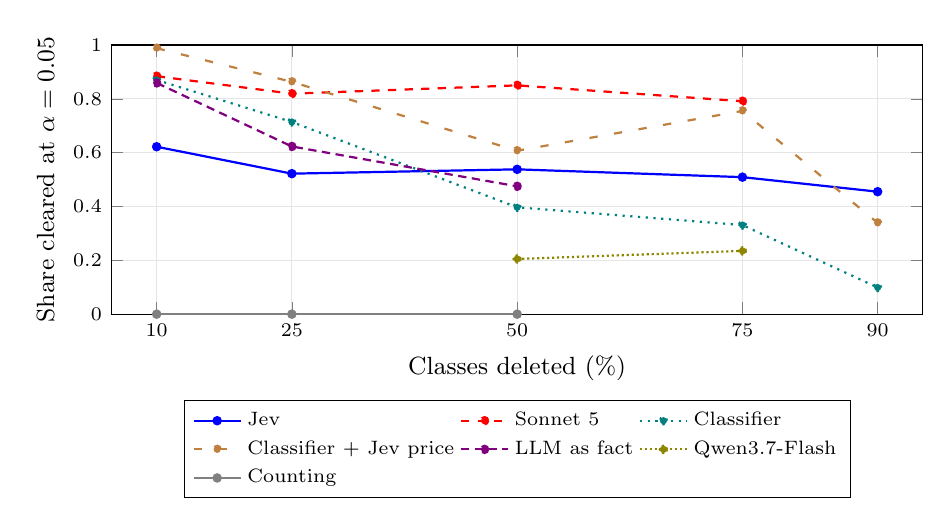
\begin{tikzpicture}
\begin{axis}[width=0.98\linewidth, height=5cm, xmin=5, xmax=95, ymin=0, ymax=1,
  xlabel={Classes deleted (\%)}, ylabel={Share cleared at $\alpha=0.05$}, xtick={10,25,50,75,90},
  legend style={font=\scriptsize, at={(0.5,-0.32)}, anchor=north}, legend cell align=left, legend columns=3,
  tick label style={font=\scriptsize}, label style={font=\small}, grid=major, grid style={gray!20}]
\addplot[blue, thick, mark=*, mark size=1.3pt] coordinates {(10,0.6220) (25,0.5220) (50,0.5380) (75,0.5090) (90,0.4550)};
\addlegendentry{Jev}
\addplot[red, thick, dashed, mark=*, mark size=1.3pt] coordinates {(10,0.8840) (25,0.8190) (50,0.8500) (75,0.7910)};
\addlegendentry{Sonnet~5}
\addplot[teal, thick, dotted, mark=*, mark size=1.3pt] coordinates {(10,0.8700) (25,0.7140) (50,0.3970) (75,0.3310) (90,0.0990)};
\addlegendentry{Classifier}
\addplot[brown, thick, loosely dashed, mark=*, mark size=1.3pt] coordinates {(10,0.9880) (25,0.8630) (50,0.6070) (75,0.7550) (90,0.3390)};
\addlegendentry{Classifier + Jev price}
\addplot[violet, thick, densely dashed, mark=*, mark size=1.3pt] coordinates {(10,0.8590) (25,0.6230) (50,0.4750)};
\addlegendentry{LLM as fact}
\addplot[olive, thick, densely dotted, mark=*, mark size=1.3pt] coordinates {(50,0.2050) (75,0.2350)};
\addlegendentry{Qwen3.7-Flash}
\addplot[gray, thick, mark=*, mark size=1.3pt] coordinates {(10,0.0000) (25,0.0000) (50,0.0000)};
\addlegendentry{Counting}
\end{axis}
\end{tikzpicture}

\caption{Whole-class deletion: share of the leak-free hard slice cleared at $\alpha=0.05$ against the share of FlowDroid-modeled classes deleted (mean over three seeds; one seed at 90\%). Held-out apps with a wrong clearance stay at or below 1.6\% in every cell.}
\label{fig:deletion}
\end{figure}

\begin{table}[t]
\caption{Ranking quality is not what certification rewards. AUROC of the bound (real flows against leak-free sinks, all verdicts), and the certified result over 200 half splits.}
\label{tab:rank}
\small
\begin{tabular}{@{}llrrrr@{}}
\toprule
Key & Pricer & AUROC & Cleared, $\alpha{=}0.05$ & Wrong, mean / p95 & Cleared, $\alpha{=}0.10$\\
\midrule
Main key & Jev & 0.970 & 48.7\% & 0.9\% / 5.8\% & 59.9\%\\
 & Sonnet~5 & 0.950 & 16.7\% & 0.0\% / 0.0\% & 16.6\%\\
 & Classifier & 0.965 & 24.3\% & 1.1\% / 4.5\% & 27.9\%\\
 & Frequency prior & 0.932 & 19.0\% & 0.0\% / 0.0\% & 18.8\%\\
 & Counting & 0.848 & 0.0\% & 0.0\% / 0.0\% & 0.0\%\\
\midrule
K2 (code-derived) & Jev & 0.999 & 93.1\% & 1.3\% / 3.1\% & 94.0\%\\
 & Sonnet~5 & 0.997 & 95.9\% & 1.6\% / 3.8\% & 96.5\%\\
 & Classifier & 0.998 & 42.5\% & 1.5\% / 6.1\% & 90.8\%\\
\bottomrule
\end{tabular}

\end{table}
Table~\ref{tab:rank} explains why pricers trade places.
Sonnet~5 ranks verdicts better than Jev on average (AUROC 0.942 against 0.855) yet clears less at $\alpha=0.05$: certification rewards only the low-bound end of the ranking, where a single real flow priced low in an app is enough to make the app wrong.
A pricer for receipts must therefore be judged by its risk-coverage curve near the origin, not by an average ranking score.
\tabph{6.5cm}{tab:panel}{Pricer panel: other model families under the same procedure.}{Rows: Jev, Sonnet~5, Qwen3.8-27B, Qwen3.7-Flash, DeepSeek-V4-Flash, GPT-5.6-luna, Gemini-3.5-Flash-Lite; columns: price (\$ per corpus), main key at $\alpha{=}0.05/0.10$, K2, deletion 50\%/75\%, AUROC against FlowDroid labels. Source: \texttt{bench/queues/panel\_*.sh} (\textbf{scheduled, running}).}

\subsection{RQ4: How good is the answer key behind the clearances?}
\label{sec:rq4}
All verdicts accepted at the chosen threshold rest on 446 distinct library facts (Table~\ref{tab:facts}).
A first, loosely worded AI pass disagreed with the key on 85 facts; a written, stricter rule (ordinary documented behavior, no custom overrides, influence is not a flow) resolved 86 of its 95 positives, and agreement with the key rose from 78\% to 97.7\%.
Because that rule was written after seeing the first pass, we report both.
A person read the Android source for the 9 positives and the 18 undecided facts (all 9 confirmed; 11 of 18 became negative) and for 40 facts the AI called negative (12 chosen for impact, 28 at random): 4 were flows, all of the kind where the method keeps a reference to its argument; the estimated miss rate among the AI's negatives is about 11\% (95\% interval 2--28\%).
Calibrating under the key with all of these answers is identical to the main key to the last digit (39.4\% cleared, 2.0\% wrong), because every path through those facts also needs another candidate flow the key keeps absent.
K2 decides 176 of the 446 facts (45\% of their use), all as no flow, and agrees with the key on 173; it is not a perfect witness (it misses the prefix flow in \texttt{File.createTempFile}).
\tabph{4.8cm}{tab:audit}{The audit in numbers: passes, answers and agreement.}{Rows: first pass, strict recheck, unsure rows resolved, person's 27 flagged facts, person's 40-fact sample, K2; columns: yes/no/unsure counts, agreement with the key, effect on the accepted verdicts. Source: \texttt{FINDINGS.md} \S16, \S19, \S21 (\textbf{have}). \textbf{Missing}: a second person on 20 facts for an agreement statistic.}

\subsection{RQ5: How faithful is our analysis to FlowDroid?}
\label{sec:rq5}
On the 37 of 40 apps where FlowDroid gave an answer (17 found no leak, 8 stopped at its own memory limit), it reports 84 leaking sink methods; our analysis reaches 56 (67\%) with every hole on and 50 (60\%) under the key; excluding 7 sinks in FlowDroid's synthetic entry method, 73\%.
The misses are mostly inter-component sinks (\texttt{startActivityForResult}, \texttt{bindService}), file and network calls, and code in bundled libraries.
In the other direction we are far less precise: we flag 4{,}514 key-true sink methods, and FlowDroid also reports 50 (1\%).
Restricting the analysis to code reachable from entry points removes only 11.5\% of these (3{,}994 remain) and does not change the recall, so dead code is not the cause; the whole-program, context-insensitive design is.
\tabph{3.8cm}{tab:fd}{Our analysis against FlowDroid at the level of sink-containing methods.}{Rows: original analysis, entry-restricted analysis (and, if built, a more precise variant); columns: FlowDroid's leaks found with all holes on, found under the key, our key-true sink methods, share FlowDroid also reports; 40 apps now, 80 apps scheduled. Source: \texttt{bench/flowdroid\_compare.py} (\textbf{have}; extension \textbf{scheduled}).}

\subsection{RQ6: What does it cost?}
\label{sec:rq6}
See Table~\ref{tab:cost}.
Building the graphs dominates (14\,h for 183 apps on 8 cores); evaluation of all 332 apps took 3.5 to 7 hours per pricing before the min-cut contraction, which is about 25 times faster on the heaviest apps \todo{measured time of a full run after contraction}; calibration takes seconds; pricing costs between \$0.2 and \$16 per corpus depending on the model.

\subsection{RQ7: Do the validity checks hold up?}
\label{sec:rq7}
\paragraph{The unit of the guarantee.}
Table~\ref{tab:unit} compares calibration units on the same bounds.
Conformal selection over verdicts with leave-one-app-out p-values and Benjamini--Hochberg~\cite{conformalselection} meets its target on this corpus (2.6\% of selected verdicts wrong at a 5\% target; on our first, smaller corpus it did not: 7.9\%) and clears more (55.6\%).
But its wrong verdicts are spread out: 166 of the 324 apps (51\%) contain at least one wrong clearance, and 62 (19\%) even at a 1\% target.
Per-program calibration leaves a wrong clearance in 1.0\% of held-out apps.
Using the bound at face value ($\delta=\alpha$, no calibration) is safe here but clears only 5.5\%: Jev's prices are conservative, and calibration recovers what they leave on the table.
\begin{table}[t]
\caption{Calibration unit and sensitivity (Jev, main key, $\alpha=0.05$). Cleared: share of the leak-free hard slice; wrong: share of (held-out) apps with at least one wrong clearance. Brackets: 5th--95th percentile over 200 splits.}
\label{tab:unit}
\small
\begin{tabular}{@{}lll@{}}
\toprule
Procedure & Cleared & Apps wrong\\
\midrule
Bound at face value, $\delta=\alpha$ (all apps) & 5.5\% & 0 of 324\\
Verdict-level conformal selection, FDR 1\% & 47.4\% & 62 of 324 (19\%)\\
Verdict-level conformal selection, FDR 5\% & 55.6\% & 166 of 324 (51\%)\\
Verdict-level conformal selection, FDR 10\% & 59.2\% & 196 of 324 (60\%)\\
\midrule
Per program (ours), $\varepsilon=0.1$, 50\% calibration & 40.0\% [37.4, 42.9] & 1.0\% [0.0, 1.9]\\
\quad $\varepsilon=0.05$ / $0.2$ & 40.0\% / 40.0\% & 1.0\% / 1.0\%\\
\quad 30\% / 70\% calibration & 38.7\% / 39.9\% & 0.9\% / 0.9\%\\
\quad apps sharing libraries kept together & 39.7\% [37.0, 42.4] & 0.9\% [0.0, 1.9]\\
\bottomrule
\end{tabular}
\end{table}
The grouped splits link apps that share at least three third-party package prefixes and keep each cluster on one side (196 clusters, the largest with 57 apps); the result does not change, so shared libraries do not inflate it.
\paragraph{Min-cut optimality.}
Solving the exact ``any correlation'' problem as a linear program over all $2^m$ worlds on 190 random graphs with 5 to 11 hole edges gives the max-flow value to within $2\cdot10^{-15}$, while the probability under independence is lower by 0.08 to 0.17 on average, so an independence-based bound understates the risk.
\paragraph{How many calibration apps are needed.}
With no wrong app among $n$ calibration apps, the exact test certifies $\alpha$ only if $(1-\alpha)^n\le\varepsilon$, so $n\ge\ln\varepsilon/\ln(1-\alpha)$: 22 apps for $\alpha=0.1$, 45 for $0.05$ and 114 for $0.02$ (Corollary~\ref{cor:n}).
Figure~\ref{fig:learning} shows that the certified clearance jumps from nothing to its full value exactly at these sizes and is flat afterwards: beyond the floor, more calibration apps do not buy more clearance, they only tighten the spread.
\begin{figure}[t]
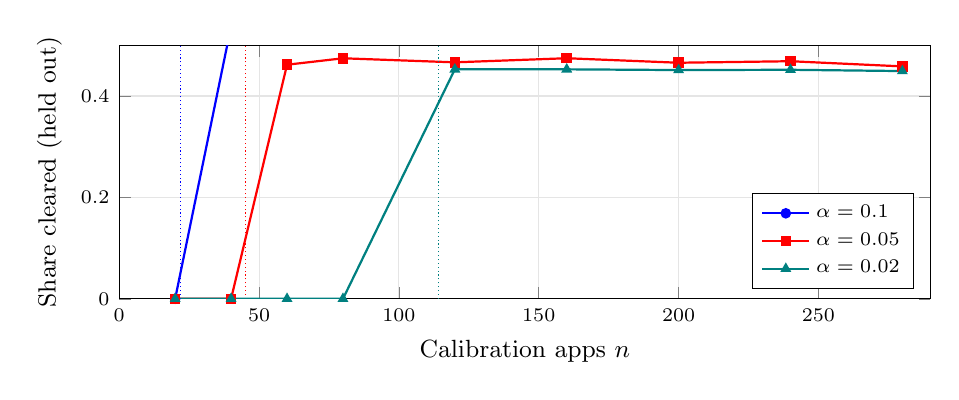
\begin{tikzpicture}
\begin{axis}[width=0.98\linewidth, height=4.8cm, xmin=0, xmax=290, ymin=0, ymax=0.5,
  xlabel={Calibration apps $n$}, ylabel={Share cleared (held out)},
  legend style={font=\scriptsize, at={(0.98,0.04)}, anchor=south east}, legend cell align=left,
  tick label style={font=\scriptsize}, label style={font=\small}, grid=major, grid style={gray!20}]
\addplot[blue, thick, mark=*, mark size=1.5pt] coordinates {(20,0.0000) (40,0.5376) (60,0.5365) (80,0.5642) (120,0.5837) (160,0.5824) (200,0.5952) (240,0.5963) (280,0.6015)};
\addlegendentry{$\alpha=0.1$}
\addplot[blue, densely dotted, thin, forget plot] coordinates {(22,0) (22,0.5)};
\addplot[red, thick, mark=square*, mark size=1.5pt] coordinates {(20,0.0000) (40,0.0000) (60,0.4618) (80,0.4745) (120,0.4665) (160,0.4746) (200,0.4657) (240,0.4687) (280,0.4585)};
\addlegendentry{$\alpha=0.05$}
\addplot[red, densely dotted, thin, forget plot] coordinates {(45,0) (45,0.5)};
\addplot[teal, thick, mark=triangle*, mark size=1.5pt] coordinates {(20,0.0000) (40,0.0000) (60,0.0000) (80,0.0000) (120,0.4527) (160,0.4527) (200,0.4513) (240,0.4518) (280,0.4493)};
\addlegendentry{$\alpha=0.02$}
\addplot[teal, densely dotted, thin, forget plot] coordinates {(114,0) (114,0.5)};
\end{axis}
\end{tikzpicture}

\caption{Certified clearance (Jev, main key) against the number of calibration apps, tested on the remaining apps (mean of 200 draws). Dotted lines: the smallest $n$ at which the exact test can certify each $\alpha$.}
\label{fig:learning}
\end{figure}

\subsection{RQ8: Which design choices matter?}
\label{sec:rq8}
\paragraph{How prices combine.}
With the same cuts and the same calibration, the sum over cut edges clears 40.0\%, the sum over distinct facts 43.0\%, the largest single price 46.8\%, and the independence product 45.3\%, all with at most 1.9\% of held-out apps wrong.
Validity comes from the calibration, not from the union bound; the union bound buys an interpretation, and counting each fact once is valid and free.
\paragraph{Question wording.}
Stating the flow rule in the pricer's question lifted clearance on the first corpus from 15.9\% to 41.1\% at $\alpha=0.10$.
\tabph{3.6cm}{tab:wording}{Question wording: Jev with three wordings.}{Rows: ``taint'' (no-answer type), ``choice'', ``choice with the object convention''; columns: AUROC/ECE on FlowDroid-modeled atoms, main key at $\alpha{=}0.05/0.10$. Source: \texttt{bench/queues/panel\_*.sh} (\textbf{scheduled}).}

\subsection{RQ9: Does the pricer hold up on code it knows less well?}
\label{sec:rq9}
\tabph{4.4cm}{tab:thirdparty}{Pricer quality on third-party libraries (less likely memorized).}{StubDroid summaries generated for OkHttp, Gson, Guava, Commons-Lang/IO, Jsoup, Retrofit; columns: AUROC, ECE, share priced below 0.05 that are real, per library and per pricer. \textbf{Missing}: build the question set (about 1{,}500 questions) with the K2 machinery and price it with Jev and the panel.}

\subsection{RQ10: Does it matter for real leaks?}
\label{sec:rq10}
\tabph{4.4cm}{tab:taintbench}{Documented leaks through library code in a real-malware benchmark.}{TaintBench apps with documented flows: how many documented flows our analysis finds with holes closed and open, how many pass through unmodeled library methods, the receipt price of those that need holes, and what FlowDroid finds. \textbf{Missing}: download the benchmark, run extraction and analysis.}

\section{Discussion}
\label{sec:discussion}
\paragraph{Lessons.}
(1)~Calibrate on programs, not on verdicts: a verdict-level false-discovery rate of a few percent still leaves a wrong clearance in most apps, because the wrong verdicts are spread over apps; per-program calibration bounds what a user of one report cares about.
(2)~State the flow rule in the question: a pricer that reads ``derived data'' narrowly under-prices getters and concentrates wrong clearances on a few widely bundled facts.
(3)~Validity and power separate cleanly: every pricer and every way of combining prices met the target; what a better pricer buys is a larger cleared share.
(4)~A key must be tested against the library code: a learned pricer looks excellent on a key built from the same conventions and fails when the classes it learned from are removed.
(5)~Counting assumptions is not a substitute for pricing them: with no prices, even receipts of one fact are unsafe in 93\% of the apps, and on malware they would clear 22 documented leaks.
(6)~Receipts are worth checking: a handful of facts sits under thousands of verdicts, so a few checks chosen by how many uncleared verdicts they block buy more than a better pricer would, and they also turn priced assumptions into reported leaks.
(7)~A pricer must be judged at the low end: models that answer almost only 0.02 or 0.95 rank well on average but put some real flows at the lowest price, and calibration then refuses them.

\paragraph{What the results mean for practice.}
An analysis designer who ships an unsound taint analysis can ship with it a list of the library assumptions behind each clean verdict and a threshold whose risk was measured on held-out apps, at a price of about \$0.4 to \$16 per corpus, and a short list of facts whose checking would clear the most.
The honest limit is that the certificate speaks about library holes, not about the rest of the analysis (Section~\ref{sec:rq5}).

\section{Threats to Validity}
\label{sec:threats}
\emph{Answer key.}
The main key contains language-model labels; K2 is code-derived but partial, uses FlowDroid's summaries for JDK leaf methods, and is not sound; the audit is AI-assisted except for 67 facts read by one person, and it checks the facts behind the clearances, not the rejected verdicts.
\emph{Exchangeability.}
Apps that bundle the same library are not independent; Section~\ref{sec:rq7} reports grouped splits.
\emph{Corpus.}
Small F-Droid apps, with half of the large ones failing to build, and 33 TaintBench malware apps; no Play Store apps. The transfer to malware rests on 31 apps, too few to estimate a risk near 5\% precisely; it shows no sign of failure, not a second guarantee.
\emph{The analysis.}
Section~\ref{sec:rq5} shows it differs from FlowDroid in both directions; the guarantee is about library holes relative to our analysis.
\emph{Pricers.}
Every pricer is a language model or a classifier trained on FlowDroid's labels; the main pricer is proprietary, and the panel (Section~\ref{sec:rq3}) includes open-weight models. Language-model answers obtained through hosted services may change over time; all prices are stored in the artifact. A few methods were priced through a different access path to the same model (152 of 17{,}830 for one panel model).
\emph{Checks.}
In RQ9 the key plays the person who checks facts, so the gain assumes checks that agree with the key; a person disagrees with it on some facts (Section~\ref{sec:rq4}).
\emph{Definition.}
Results depend on the flow definition; the one choice that mattered (reference keeping) is reported under both readings.
\emph{Construct.}
A ``wrong clearance'' is relative to the key; no key is ground truth.

\section{Related Work}
\label{sec:related}
\paragraph{Minimal assumptions behind a verdict.}
Bastani et al.~\cite{bastani-oopsla15} compute min-cuts in a source-sink flow graph, each cut a set of statements assumed unreachable, and ask a developer to confirm them with tests; Zhu et al.~\cite{zhu-aplas13} abduce the library specifications needed to verify a source-sink property; Dillig et al.~\cite{dillig-pldi12} and Elrond~\cite{elrond} abduce proof obligations or specifications.
Our receipt is their cut with prices; the human becomes optional, a calibrated prior carries the rest with a certified error, and when a person does check facts, receipts tell which few facts unlock the most verdicts (RQ9).
\paragraph{Library specification inference.}
Merlin~\cite{merlin} infers specifications with probabilities but thresholds them into facts; Seldon~\cite{seldon}, StubDroid~\cite{stubdroid}, Atlas~\cite{atlas} and Bastani et al.~\cite{bastani-popl15} produce specifications without a verdict-level error; LLM-based extraction~\cite{iris,semtaint} takes the model's answers as fact.
We use StubDroid as an independent key and the model-as-fact approach as a baseline.
\paragraph{Probabilistic inference.}
Praline~\cite{praline} computes sound probability bounds for Datalog outputs under partly known input correlations; on a reachability fragment with only marginals known, its optimum equals the min-cut (Proposition~\ref{prop:tight}), which we use because it is a max-flow.
\paragraph{Neuro-symbolic analysis.}
NeuroLog~\cite{neurolog} feeds model-extracted facts to Datalog to find bugs; we use the same kind of stack to bound missed flows rather than to find them.
\paragraph{Risk control.}
The calibration is Learn-then-Test~\cite{lt}; conformal selection~\cite{conformalselection} is the verdict-level alternative; it controls the false-discovery rate among selected verdicts, which here leaves wrong clearances in most apps.
\paragraph{Benchmarks.}
TaintBench~\cite{taintbench} documents real malware leaks with their paths; we use it to ask how many of them depend on library holes and whether a threshold certified on benign apps transfers.
\paragraph{Soundiness.}
The soundiness manifesto~\cite{soundiness} asks analyses to list what they leave out; receipts make one such list checkable per verdict and attach a risk to it.

\section{Conclusion}
\label{sec:conclusion}
An unsound static analysis can be $(\alpha,\varepsilon)$-soundy: it can say on which library assumptions each clean verdict rests, and clear verdicts with an error rate over programs that is certified, not hoped for.
The certificate holds for every pricer we tried; a good pricer buys clearance, a few well-chosen checks of receipt facts buy more, and on real malware the threshold certified on benign apps transferred.
The limits are as clear: our analysis is a weaker tool than FlowDroid, the key is only partly independent of language models, and cheap models price too confidently to help.


\section*{Disclosure of Generative AI Use}
Generative AI is part of the method and of the production of this paper, and we disclose both.
\emph{In the method:} language models price candidate library flows (a proprietary calibrated model, Sonnet~5, and a panel of other models), one language model wrote the labels the main answer key uses for methods FlowDroid does not model, and AI-assisted passes labeled the library facts of the audit (Section~\ref{sec:setup}); a person read the source for 67 facts and for a sample of the rest.
\emph{In the artifact and the paper:} an AI coding assistant wrote and ran much of the analysis, evaluation and experiment code under the authors' direction, and drafted parts of the text and tables from the authors' notes and logs.
The authors define the research questions and the flow definition, decided which experiments to run, checked the reported numbers against the logs and result files, and take responsibility for the content.
\todo{Name the tools and versions exactly as the ACM policy requires, and confirm the wording with all authors before submission.}


\section*{Data Availability}
\todo{Replace with the anonymous link (e.g.\ anonymous.4open.science) to the artifact before submission.}
The artifact contains (i)~the extraction and Datalog analysis (Soot facts, Souffl\'e program, graph builder), (ii)~the min-cut evaluation and the calibration code, with the scripts that regenerate every table and figure from the stored result files, (iii)~the stored flow graphs of the 332 apps (about 1\,GB), the per-sink results for every pricer and key, and the price files of every pricer, (iv)~the answer keys (FlowDroid's summaries, the language-model labels, the StubDroid summaries and logs, the deletion-benchmark generator), (v)~the audit: the fact lists, all answers with reasons and the person's source check, and the written instructions given to labelers, and (vi)~the FlowDroid runs with and without its library summaries.
The list of F-Droid app versions is included; the APKs are downloaded from F-Droid by a script.
The proprietary pricer (Jev) cannot be redistributed: its prices for every method are included as files, and the pricers based on open-weight models can be rerun from the scripts (Section~\ref{sec:rq3}).
The labels written by hosted language models are included as files, since a hosted model's answers may change over time.
\todo{State the license and the archival repository (Zenodo or similar) for the camera-ready version.}


\bibliographystyle{ACM-Reference-Format}
\bibliography{refs}

\appendix
\section{Flow Definition and Labeling Rubric}
\label{app:flow}
Labelers were given the following question for every fact: method $M$ is called with $X$ holding a secret; after the call, is a piece of the secret in $Y$?
A flow exists if $X$'s data is copied or computed into $Y$ (code C), stored in $Y$ as the method's purpose, including a reference to it (S), or $Y$ is read out of $X$, including its size, emptiness or metadata (R).
It is not a flow if $X$ only picks which existing thing is used (P), only controls how much, when or whether (K), changes only incidental state such as caches or back-pointers (I), matters only through a custom override, callback, other OS version or unusual argument (H), or has no connection (N); an undecidable case is U.
Every answer carried a one-sentence mechanism and, for the person's pass, the evidence (line or called method).
\tabph{4.0cm}{tab:rubric}{The reason codes and a worked example for each.}{Nine codes C, S, R, P, K, I, H, N, U with one real example each (e.g.\ \texttt{String.substring} receiver $\to$ return: C; start index $\to$ return: P). Source: \texttt{AUDIT\_RECHECK.md} (\textbf{have}).}

\section{Proof Details}
\label{app:proofs}
\todo{Write out Proposition~\ref{prop:tight} with the flow-decomposition and padding construction for graphs with parallel edges and edges of probability one, and Proposition~\ref{prop:ltt} with the exact binomial p-value and the fixed-sequence argument, including why monotonicity of $L$ is needed only for the choice of order.}

\section{Additional Results}
\label{app:results}
\tabph{6cm}{tab:app-deletion}{Method-level and class-level deletion at all rates, both targets, every pricer, with the worst seed.}{Full tables behind Figure~\ref{fig:deletion}. Source: \texttt{k1\_summary\_final\_*.log}, \texttt{k1c\_summary\_final\_*.log} (\textbf{have}).}
\tabph{6cm}{tab:app-fd}{Per-app FlowDroid comparison (leaks found, missed, states).}{One row per app. Source: \texttt{bench/flowdroid\_compare.py}, \texttt{bench/flowdroid\_none\_compare.py} (\textbf{have}).}
\tabph{5cm}{tab:app-keys}{Calibration per key at $\alpha\in\{0.02,0.05,0.10\}$, with the chosen threshold in each split.}{Source: \texttt{ltt\_*.log} (\textbf{have}; panel pending).}

\end{document}
